\section{Gefahren der Nebenläufigkeit}
Neue Arten von Programmierfehler, die es bei single-Threading nicht gibt. 
Können sporadisch oder selten auftreten.
Sehr schwierig durch Tests zu finden.

\subsection{Race Condition}
Mehrere Threads greifen auf gemeinsame Ressourcen ohne genügend synchronisation zu.
Mögliche falsche Resultate oder falsches Verhalten.
Ursache oft ein Data Race, nicht immer.

\subsubsection{Data Race}
Unsynchronisierter Zugriff auf gleichen Speicher.
Selbe Variable oder Array Element (min. 1 schreibender Zugriff).

\subsubsection{Race Condition ohne Data Race}
Critical Sections nicht geschützt. 
Data Races mit Synchronisation eliminiert, aber nicht genügend grosse synchronisierte Blöcke.
\begin{lstlisting}
synchronized int getBalance() { return balance; }
synchronized void setBalance(int x) { balance = x; }
// Mehrere Threads, Kein Atomares Inc - Lost Update moeglich 
accout.setBalance(account.getBalance() + 100);
\end{lstlisting}

\subsubsection{Kombinationen}
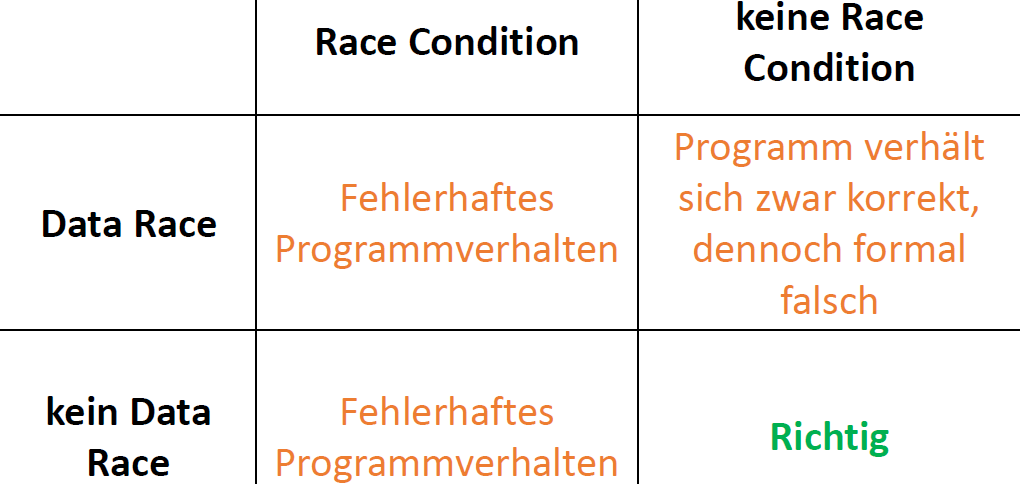
\includegraphics[width=0.6\linewidth]{img/race_condition.png}\\ 
\textbf{Alles Synchronisieren?} Hilft nichts. Race Condition trotzdem möglich. Weitere Nebenläufigkeitsfehler.
Synchronisationskosten sind relativ teuer.

\subsection{Synchronisation: Verzichtbare Fälle}
\textbf{Immutability (Unveränderlicheit):} Objekte mit nur lesendem Zugriff.
\textbf{Confinement (Einsperrung):} Objekt gehört nur einem Thread zu einer Zeit.

\subsubsection{Immutable Objects}
Instanzvariablen alle \textit{final}. Primitive Datentypen. Referenzen wiederum auf Immutable Objekte.
Methoden mit nur lesendem Zugriff. Konstruktor initialisiert Instanzvariablen.
Nach Konstruktor kann Objekt ohne Synchronisation von Threads verwendet werden.

\subsubsection{Confinement}
Struktur garantiert, dass auf ein Objekt nur durch einen Thread zur gleichen Zeit zugegriffen wird.
\textbf{Thread Confinement:} Objekt gehört nur einem Thread und wird nur von demjenigen verwendet.
\textbf{Object Confinement:} Objekt in anderem bereits synchronisierten Objekt eingekapselt.\\ 
\textbf{Kapselungsbrüche:} 1. Inneres Objekt ist aussen zugreifbar. 2. Rückgabe einer Referenz auf inneres Objekt.
3. Holder installiert selber Referenz ausserhalb. 4. Inneres Objekt gibt selber \textit{this} raus.


\subsection{Thread Safety}
Klassen / Methoden, die intern synchronisiert sind. Keine Race Conditions innerhalb dieses Codes.
Kritischer Abschnitt nur pro Methode erfüllt.
\textbf{Aber:} Kein kritischer Abschnitt über mehrere Methodenaufrufe. 
Andere Nebenläufigkeitsfehler möglich.

\subsubsection{Java Collections - Thread Safety}
Alte Java 1.0 Collections (Vector, Stack, Hashtable): \textbf{JA}. 
Moderne Collections (HashSet, TreeSet, ArrayList, etc.): \textbf{NEIN}.
Concurrent Collections (ConcurrentHashMap, etc.): \textbf{JA}.

\subsection{Verstecktes Multi-Threading}
\textbf{Finalizers:} Laufen über separaten Finalizer-Thread.
\textbf{Timers:} Handler durch separaten Thread ausgeführt (ausser GUI).
\textbf{Externe Libraries \& Frameworks:} z.B. Abarbeitung von Web-Service Aufrufen.

\subsection{Deadlock}
Beide Threads sperren sich gegenseitig aus:
\begin{lstlisting}
syncrhonized(listA) { // Thread 1
    syncrhonized(listB) {
        listB.addAll(listA);
    }
}
synchronized(listB) { // Thread 2
    synchronized(listA) {
        listA.addAll(listB);
    }
}
\end{lstlisting}

\subsubsection{Spezialfall: Livelocks}
Threads haben sich gegenseitig permanent blockiert. Führen aber noch Warteinstruktionen aus.
Verbrauchen CPU während Deadlock.
\begin{lstlisting}
// Thread 1
b = false; while (!a) { } b = true;
// Thread 2
a = false; while (!b) { } a = true;
\end{lstlisting}

\subsubsection{Deadlock Erkennung}
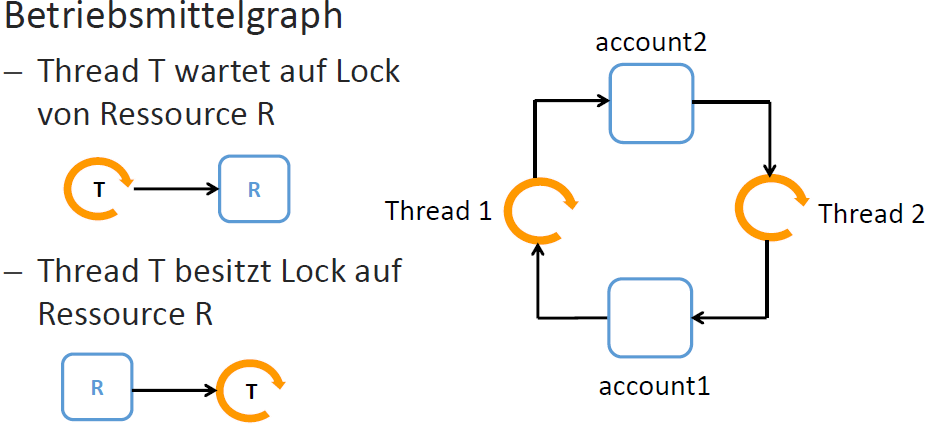
\includegraphics[width=0.7\linewidth]{img/betriebsmittelgraph.png}\\
\textit{Deadlock = Zyklus im Betriebsmittelgraph}\\ 
\textbf{Deadlock Voraussetzungen:} Geschachtelte Locks, Zyklische Warteabhänigkeiten

\subsubsection{Deadlock Vermeidung}
\textbf{Lineare Sperrordnung} der Ressourcen einführen. 
Nur geschachtelt in aufsteigender Reihenfolge sperren. 
Eliminiert zyklische Warteabhänigkeiten.\\ 
\textbf{Grobgranulare Locks} wählen.
Wenn lineare Sperrordnung nicht möglich/sinvoll ist.
Sperre gesamte Bank bei Kontenzugriff.
Eliminiert Schachtelung von Locks.

\subsection{Starvation}
Ein Thread kriegt nie die Chance, auf eine Ressource zuzugreifen, obwohl sie immer wieder frei wird.
Andere Threads überholen andauernd. Liveness/Fairness Problem.
\begin{lstlisting}
do { // Starvation moeglich 
    success = account.widthdraw(100);
} while (!success);
\end{lstlisting}

\subsubsection{Vermeidung}
Faire Synchronisationskonstrukte (bei Semaphore, Lock \& Condition, ReadwriteLock möglich).
Java Monitor hat ein Fairness Problem (Starvation anfällig).

\subsection{Parallelität Korrektheitskriterien}
\textbf{Safety:} Keine Race Conditions, Keine Deadlocks.
\textbf{Liveness:} Keine Starvation.